\documentclass[tikz,border=8pt]{standalone}
\usetikzlibrary{arrows.meta,positioning}
\begin{document}
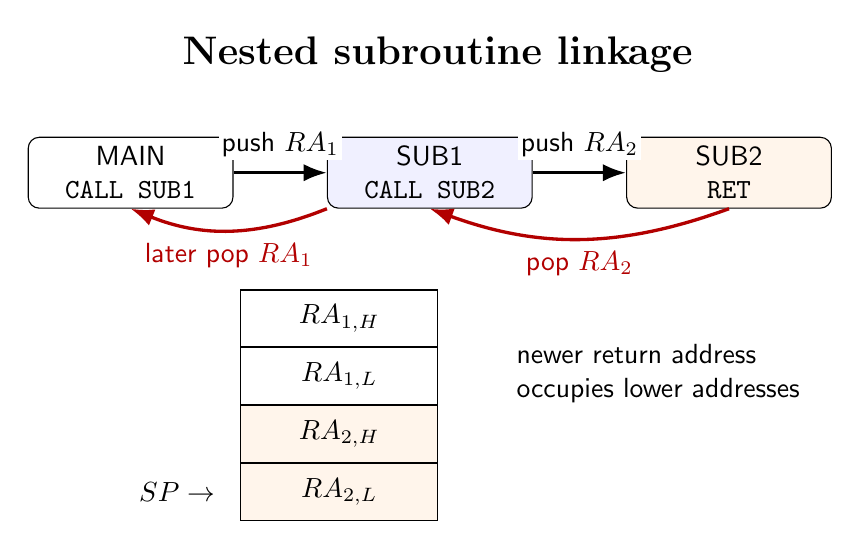
\begin{tikzpicture}[font=\sffamily,>=Latex,code/.style={draw,rounded corners,minimum width=2.6cm,minimum height=.9cm,align=center},cell/.style={draw,minimum width=2.5cm,minimum height=.72cm}]
\node[font=\Large\bfseries] at (5.4,5.2) {Nested subroutine linkage};
\node[code] (main) at (1.5,3.7) {MAIN\\\texttt{CALL SUB1}};
\node[code,fill=blue!6] (s1) at (5.3,3.7) {SUB1\\\texttt{CALL SUB2}};
\node[code,fill=orange!8] (s2) at (9.1,3.7) {SUB2\\\texttt{RET}};
\draw[very thick,->] (main)--(s1)
  node[midway,above=4pt,fill=white,inner sep=1pt] {push $RA_1$};
\draw[very thick,->] (s1)--(s2)
  node[midway,above=4pt,fill=white,inner sep=1pt] {push $RA_2$};
\node[cell] (ra1h) at (4.15,1.85) {$RA_{1,H}$};
\node[cell,below=0pt of ra1h] (ra1l) {$RA_{1,L}$};
\node[cell,below=0pt of ra1l,fill=orange!8] (ra2h) {$RA_{2,H}$};
\node[cell,below=0pt of ra2h,fill=orange!8] (ra2l) {$RA_{2,L}$};
\node[left=2mm of ra2l] {$SP\to$};
\draw[very thick,red!70!black,->] (s2.south) to[bend left=20]
  node[midway,below=3pt,fill=white,inner sep=1pt] {pop $RA_2$} (s1.south);
\draw[very thick,red!70!black,->] (s1.south west) to[bend left=22]
  node[midway,below=3pt,fill=white,inner sep=1pt] {later pop $RA_1$} (main.south);
\node[align=left] at (8.2,1.15) {newer return address\\occupies lower addresses};
\end{tikzpicture}
\end{document}
